\epigraph{Slow is smooth, and smooth is fast}
{\textit{Military proverb}}

\section{Speed vs Accuracy}

As much as this challenge rewards speed, it also rewards accuracy. In the later challenges especially, I often found that acting too quickly meant committing to an idea before the problem had been properly understood. When an initial idea fails, it is easy to move on to another, and then another again, without ever fully engaging with the structure of the cipher itself.

A more effective approach might be to first pause. After all, there is a reason races begin with \textit{On Your Marks... Get Set... Go!} and not just someone yelling \textit{GO!} at a group of already stressed people. The pause is not separate from the start, it's part of the start. It gives you a second to settle, to look ahead, to position yourself, and to begin with some sense of direction rather than pure adrenaline.

Codebreaking is no different. So before attempting to solve anything, it helps to take a step back and look carefully at what is actually in front of you. At this stage, your goal is not to crack the cipher, but to understand what you're dealing with.

\section{What Is Actually There}

When you look at the ciphertext as it is, ask questions about what you can see. Think of going through steps of a mental flowchart to problem solving 

Some questions you might want to consider could be: 
\begin{itemize}
    \item What characters appear? 
    \item How many distinct characters are there? 
    \item Do certain patterns in the text repeat? 
    \item Are there deliberate spaces in the text? 
\end{itemize}

These questions do not require any specialised knowledge as they are less about applying techniques, and more about paying attention to the information that is already present.


\section{Defining the Unit}

One of the most important questions you can ask yourself early on is: \textbf{What is one unit of this ciphertext? }

It might be natural to assume that each character corresponds to a letter. But ciphers are under no obligation to be that cooperative. A single symbol might represent a letter, or a pair of letters, or a number, or a code. Maybe the groupings of such symbols or characters only make sense when they appear in a certain pattern. 

For example, in Morse code, individual dots and dashes are not letters. Only when they are grouped in the correct way do they form meaningful units, so treating each symbol independently would not lead to a solution. And if you get the unit wrong, you can spend a very long time being impressively wrong in a highly committed way.

Recognising the correct unit is not always immediate. But simply knowing that this is a question worth asking can save you from making assumptions too early, which is one of the more common ways to accidentally make your own life harder.

\section{Asking Better Questions}

If there’s anything I’ve learned, it’s that quality of your thinking is determined by the quality of the questions you ask.

At the beginning of a cipher, it is easy to focus on questions that are too specific about the type of cipher. But those questions assume that you already understand the problem well enough to classify it.

More useful questions are broader and more structural such as: 
\begin{itemize}
    \item What patterns are present? 
    \item What is and isn't consistent? 
    \item What assumptions am I making? 
    \item What would have to be true for this to work? 
\end{itemize}

Notice how the questions above don't have quick answers, but they do guide your attention in a more productive direction in the sense that they help you build a clearer picture of the problem before committing to a particular approach.

The purpose of the starting line is not to immediately produce an answer, but to begin understanding the problem in a structured way. By observing carefully, questioning assumptions, and resisting the urge to act too quickly, you create the conditions for meaningful progress later on.

\begin{figure}
    \centering
    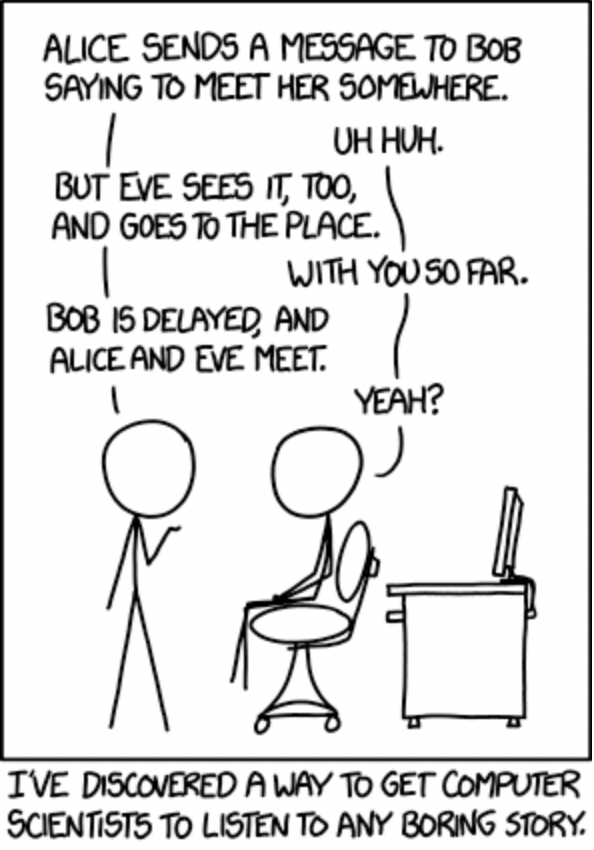
\includegraphics[width=0.5\linewidth]{xkcd/protocol.png}
    \caption{\textbf{\href{https://www.explainxkcd.com/wiki/index.php/1323:_Protocol}{1323: Protocol}}}
\end{figure}